\documentclass[border=6pt]{standalone}
%=======================================================================
%  ICCIT 2026 -- CAMERA-READY version, 6 pages, IEEE conference format
%  From Spikes to Sentences: A Hybrid CTC Decoder with Confidence-Gated
%  Language Model Rescoring
%  Compile: pdflatex x3, with revision_results.tex in this folder.
%=======================================================================

\usepackage{amsmath,amssymb}
\usepackage{graphicx}
\usepackage{booktabs}
\usepackage{multirow}
\usepackage{array}
\usepackage{xcolor}
\usepackage{tikz}
\usetikzlibrary{arrows.meta,positioning,calc,fit,backgrounds,shapes.geometric}
\usepackage{pgfplots}
\pgfplotsset{compat=1.17}
\usepackage{algorithm}
\usepackage{algpseudocode}
\usepackage{adjustbox}



\definecolor{ioFill}{HTML}{ECEFF4}\definecolor{ioLine}{HTML}{4C566A}
\definecolor{acFill}{HTML}{E3EEF9}\definecolor{acLine}{HTML}{3B6EA5}
\definecolor{reFill}{HTML}{E0F0EC}\definecolor{reLine}{HTML}{2E8B7F}
\definecolor{trFill}{HTML}{ECE6F5}\definecolor{trLine}{HTML}{6A4C93}
\definecolor{deFill}{HTML}{E6F0E1}\definecolor{deLine}{HTML}{4E8B3B}
\definecolor{llFill}{HTML}{FBEBDD}\definecolor{llLine}{HTML}{C1662F}
\definecolor{gaFill}{HTML}{FFF6E9}\definecolor{gaLine}{HTML}{B8860B}
\definecolor{inkLine}{HTML}{3B4252}

\tikzset{
  blk/.style={rounded corners=3pt,draw,line width=0.9pt,align=center,
              inner sep=4pt,font=\footnotesize},
  io/.style={blk,fill=ioFill,draw=ioLine},
  ac/.style={blk,fill=acFill,draw=acLine},
  re/.style={blk,fill=reFill,draw=reLine},
  tr/.style={blk,fill=trFill,draw=trLine},
  de/.style={blk,fill=deFill,draw=deLine},
  ll/.style={blk,fill=llFill,draw=llLine},
  gate/.style={diamond,aspect=1.7,draw=gaLine,fill=gaFill,line width=0.9pt,
               align=center,inner sep=1pt,font=\footnotesize},
  fl/.style={-{Stealth[length=5pt]},line width=0.9pt,draw=inkLine},
  dec/.style={-{Stealth[length=5pt]},line width=0.8pt,draw=deLine,dashed},
  tag/.style={font=\scriptsize\itshape,text=inkLine,fill=white,inner sep=1pt},
  capt/.style={font=\scriptsize,text=ioLine},
}

\newcommand{\pct}{\,\%}


\begin{document}
\setlength{\columnwidth}{3.5in}
\fontsize{10}{12}\selectfont
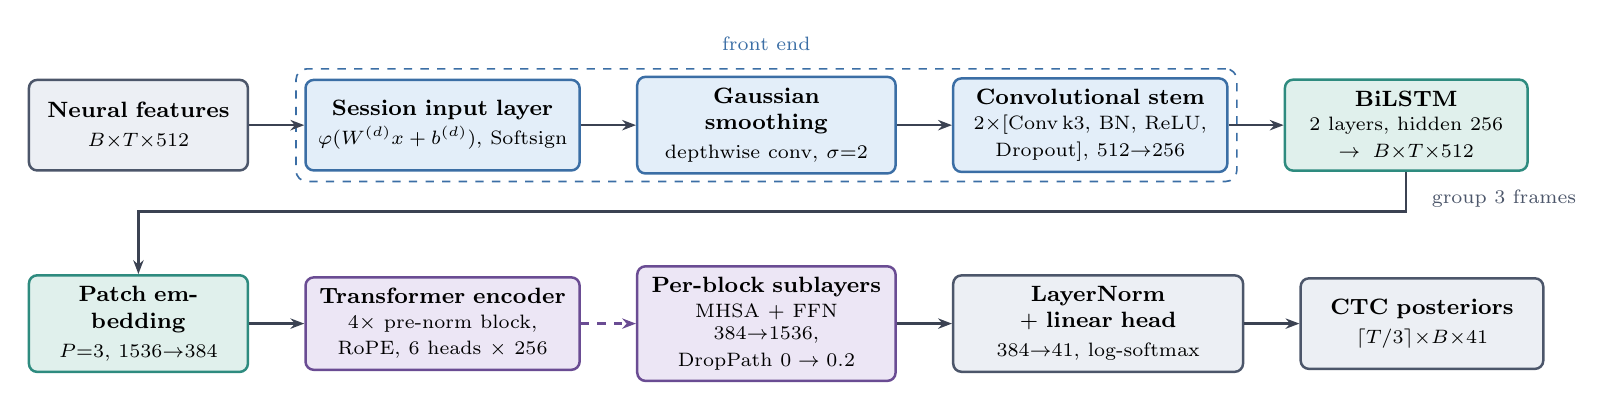
\begin{tikzpicture}[node distance=7mm]
  % ---------- row 1 ----------
  \node[io,minimum height=11.5mm,text width=25mm] (in)
       {\textbf{Neural features}\\[1pt]\scriptsize $B{\times}T{\times}512$};
  \node[ac,right=of in,minimum height=11.5mm,text width=32mm] (day)
       {\textbf{Session input layer}\\[1pt]\scriptsize $\varphi(W^{(d)}x+b^{(d)})$, Softsign};
  \node[ac,right=of day,minimum height=11.5mm,text width=30mm] (gau)
       {\textbf{Gaussian smoothing}\\[1pt]\scriptsize depthwise conv, $\sigma{=}2$};
  \node[ac,right=of gau,minimum height=11.5mm,text width=32mm] (cnn)
       {\textbf{Convolutional stem}\\[1pt]\scriptsize $2\times$[Conv\,k3, BN, ReLU,\\ Dropout], $512{\to}256$};
  \node[re,right=of cnn,minimum height=11.5mm,text width=28mm] (lstm)
       {\textbf{BiLSTM}\\[1pt]\scriptsize 2 layers, hidden 256\\ $\to B{\times}T{\times}512$};

  \foreach \a/\b in {in/day,day/gau,gau/cnn,cnn/lstm} \draw[fl] (\a) -- (\b);

  % ---------- row 2 ----------
  \node[re,below=13mm of in,minimum height=11.5mm,text width=25mm] (patch)
       {\textbf{Patch embedding}\\[1pt]\scriptsize $P{=}3$, $1536{\to}384$};
  \node[tr,right=of patch,minimum height=11.5mm,text width=32mm] (enc)
       {\textbf{Transformer encoder}\\[1pt]\scriptsize $4\times$ pre-norm block,\\ RoPE, 6 heads $\times$ 256};
  \node[tr,right=of enc,minimum height=11.5mm,text width=30mm] (ffn)
       {\textbf{Per-block sublayers}\\[1pt]\scriptsize MHSA $+$ FFN $384{\to}1536$,\\ DropPath $0\!\to\!0.2$};
  \node[io,right=of ffn,minimum height=11.5mm,text width=34mm] (head)
       {\textbf{LayerNorm $+$ linear head}\\[1pt]\scriptsize $384{\to}41$, log-softmax};
  \node[io,right=of head,minimum height=11.5mm,text width=28mm] (out)
       {\textbf{CTC posteriors}\\[1pt]\scriptsize $\lceil T/3\rceil{\times}B{\times}41$};

  \draw[fl] (patch) -- (enc);
  \draw[trLine,line width=0.9pt,dashed,-{Stealth[length=5pt]}] (enc) -- (ffn);
  \draw[fl] (ffn) -- (head); \draw[fl] (head) -- (out);

  % wrap arrow from row 1 to row 2
  \draw[fl] (lstm.south) -- ++(0,-5mm) -| (patch.north);
  \node[capt,anchor=west] at ($(lstm.south)+(2mm,-3.4mm)$)
       {\scriptsize group 3 frames};

  \begin{scope}[on background layer]
    \node[draw=acLine,dashed,rounded corners,line width=0.6pt,fit=(day)(cnn),
          inner sep=3pt] (fe) {};
  \end{scope}
  \node[capt,text=acLine,above=1mm of fe.north] {\scriptsize front end};
\end{tikzpicture}
\end{document}
